\input{../YKY-preamble.tex}
% \usepackage[no-math]{fontspec}
% \setmainfont[BoldFont=Alibaba_Sans_Regular.otf,ItalicFont=Alibaba_Sans_Light_Italic.otf]{Alibaba_Sans_Light.otf}

\usepackage[backend=biber]{biblatex}
\bibliography{../AGI-book}

\usepackage[active,tightpage]{preview}		% for continuous page(s)
\renewcommand{\PreviewBorder}{0.5cm}
\renewcommand{\thempfootnote}{\arabic{mpfootnote}}

\usepackage[absolute,overlay]{textpos}		% for page number on upper left corner

\usepackage{color}
% \usepackage{mathtools}
\usepackage[hyperfootnotes=false]{hyperref}

% \usepackage[backend=biber,style=numeric]{biblatex}
% \bibliography{../AGI-book}
% \renewcommand*{\bibfont}{\footnotesize}

\usetikzlibrary{shapes}
% \usepackage[export]{adjustbox}	% ??
\usepackage{verbatim} % for comments
% \usepackage{newtxtext,newtxmath}	% Times New Roman font

% \titleformat{\subsection}[hang]{\bfseries\large\color{blue}}{}{0pt}{} 
% \numberwithin{equation}{subsection}

\newcommand{\underdash}[1]{%
	\tikz[baseline=(toUnderline.base)]{
		\node[inner sep=1pt,outer sep=10pt] (toUnderline) {#1};
		\draw[dashed] ([yshift=-0pt]toUnderline.south west) -- ([yshift=-0pt]toUnderline.south east);
	}%
}%

\newcommand\reduline{\bgroup\markoverwith{\textcolor{red}{\rule[-0.5ex]{2pt}{0.4pt}}}\ULon}

%\DeclareSymbolFont{symbolsC}{U}{txsyc}{m}{n}
%\DeclareMathSymbol{\strictif}{\mathrel}{symbolsC}{74}
%\DeclareSymbolFont{AMSb}{U}{msb}{m}{n}
%\DeclareSymbolFontAlphabet{\mathbb}{AMSb}
%\setmathfont{lmroman17-regular.otf}
\DeclareMathOperator*{\argmin}{arg\,min}
\DeclareMathOperator*{\argmax}{arg\,max}

% \usepackage[most]{tcolorbox}
%\tcbset{on line, 
%	boxsep=4pt, left=0pt,right=0pt,top=0pt,bottom=0pt,
%	colframe=red,colback=pink,
%	highlight math style={enhanced}
%}
%\newcommand{\atom}{\vcenter{\hbox{\tcbox{....}}}}

\let\oldtextbf\textbf
\renewcommand{\textbf}[1]{\textcolor{blue}{\oldtextbf{#1}}}

\newcommand{\logic}[1]{{\color{violet}{\textit{#1}}}}
\newcommand{\underconst}{
\includegraphics[scale=0.5]{../2020/UnderConst.png}}
\newcommand{\KBsymbol}{\vcenter{\hbox{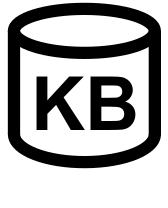
\includegraphics[scale=1]{../KB-symbol.png}}}}
\newcommand{\token}{\vcenter{\hbox{\includegraphics[scale=1]{token.png}}}}
\newcommand{\proposition}{\vcenter{\hbox{\includegraphics[scale=0.8]{proposition.png}}}}

\begin{document}

\begin{preview}

\title{}
% \title{\vspace{-0cm} \bfseries\color{blue}{\LARGE \cc{全球平等主义}{Global egalitarianism}}}

% \author{YKY} % Your name
% \date{\vspace{-2.5cm}}
\date{}
% \date{\vspace{-2.4cm} \tiny \today}

\maketitle

\vspace{-4.5cm}
\hfill{\tiny\today}
\vspace*{1.5cm}

\setcounter{section}{-1}
\newcounter{mypage}
\setcounter{mypage}{0}

% (1) Circled page number on upper left corner
%\begin{textblock*}{5cm}(2.1cm,2.3cm) % {block width} (coords) 
%{\color{red}{\large \textcircled{\small \themypage}}}
%\addtocounter{mypage}{1}
%\end{textblock*}

\begin{minipage}{\textwidth}
\setlength{\parskip}{0.4\baselineskip}

\begin{itemize}
	\item \cc{在 帝国主义 下，被欺压的人 互相出卖 是很常见的现象}{}
	
	\item \cc{最有名的是《圣经》里 犹大 出卖 耶稣}{}
	
	\item \cc{其实 基督教 本身就是对帝国主义的一种回应}{}
	
	\item \cc{以夷制夷 是利用本地人管治他们的同胞，例如英国利用印度人、或者欧洲人在美洲利用各种族互相残杀}{}
	
	\item \cc{在 殖民主义时期，由于西方的优势是 压倒性的，人们只能选择 投降 或作无谓的反抗和 牺牲。在这情况下「识时务者为俊杰」也许没有不妥？}{}
	
	\item \cc{美国的问题是 歧视 有色人种，而极权政府的问题是不尊重本国人民的人权 -- 也就是说，鄙视自己的同胞 -- 这是一种 internalized 的种族歧视，因为一直被白人鄙视而自己也逐渐觉得自己是劣等民族。}{}
	
	\item \cc{在 殖民主义 时期，西方人的优势 overwhelming (压倒性)，人们要么选择投降，要么作出没有前景的反抗。在这情况下，「识时务者为俊杰」或许没有不妥？}{}
	
	\item \cc{在印度被英国殖民之初，英国人贿赂了 军官 Mir Jafar 以推翻 Bengal 的统治者；时至今日，他的名字仍然是「卖国贼」的同义词。 人们 争相出卖同胞 以获得宠幸，成为了殖民时期的常态。}{}
	
	\item \cc{到了今天，殖民主义被普遍认为不合乎道德，然而却有 新殖民主义 (neo-colonialism) 在 隐蔽地 蔓延。究竟我们是否要屈服于新殖民主义之下，抑或现在是 多极世界格局 (multi-polar world order) 抬头的时机？ 这是一个非常考验判断力的问题。}{}
	
 	\item \cc{一方面我们看到了中国经济奇迹般的崛起、俄乌战争僵持不下、美国-伊朗战争亦胶着，令人怀疑美国是否仍有能力 支配世界？西方领先世界的局面是不是已走到一个 拐点 (inflection point / turning point)?}{}
 	
	\item \cc{另方面，中国-俄罗斯-北韩-伊朗 等 极权统治 似乎没有松懈的迹象，令这些国家 停滞不前。}{}

\end{itemize}

\end{minipage}
\end{preview}

\begin{comment}
\begin{preview}
\begin{textblock*}{5cm}(2.1cm,2.3cm) % {block width} (coords) 
	{\color{red}{\large \textcircled{\small \themypage}}}
	\addtocounter{mypage}{1}
\end{textblock*}

\begin{minipage}{\textwidth}
	\setlength{\parskip}{0.4\baselineskip}

\section{This}

\begin{itemize}
	\item Here
\end{itemize}

\end{minipage}
\end{preview}

\begin{preview}
\begin{textblock*}{5cm}(2.1cm,2.3cm) % {block width} (coords) 
{\color{red}{\large \textcircled{\small \themypage}}}
\addtocounter{mypage}{1}
\end{textblock*}

\begin{minipage}{\textwidth}
\setlength{\parskip}{0.4\baselineskip}

\section{This}

\begin{itemize}
	\item Here
\end{itemize}

\end{minipage}
\end{preview}

\begin{preview}
\begin{textblock*}{5cm}(2.1cm,2.3cm) % {block width} (coords) 
	{\color{red}{\large \textcircled{\small \themypage}}}
	\addtocounter{mypage}{1}
\end{textblock*}

\begin{minipage}{\textwidth}
	\setlength{\parskip}{0.4\baselineskip}

\section{This}

\begin{itemize}
	\item Here
\end{itemize}

\end{minipage}
\end{preview}

\end{comment}

\end{document}
